\documentclass[11pt]{amsart}
\setlength{\topmargin}{-0.3in} % usually -0.25in
\addtolength{\textheight}{1.5in} % usually 1.25in
\addtolength{\oddsidemargin}{-0.8in}
\addtolength{\evensidemargin}{-0.8in}
\addtolength{\textwidth}{1.45in} %\setlength{\parindent}{0pt}

\renewcommand{\baselinestretch}{1.05}

\usepackage{amssymb,xspace,verbatim,palatino}
\usepackage{fancyvrb}

\usepackage[pdftex, colorlinks=true, plainpages=false, linkcolor=black, citecolor=red, urlcolor=red]{hyperref}

%\usepackage[final]{graphicx}
\usepackage{graphbox}  % loads graphicx

\newtheorem*{thm}{Theorem}
\newtheorem*{lem}{Lemma}

\newcommand{\CC}{{\mathbb{C}}}
\renewcommand{\Im}{\operatorname{Im}}
\newcommand{\NN}{{\mathbb{N}}}
\newcommand{\RR}{{\mathbb{R}}}
\renewcommand{\Re}{\operatorname{Re}}
\newcommand{\ZZ}{{\mathbb{Z}}}

\newcommand{\Arg}{\operatorname{Arg}}

\newcommand{\Span}{\operatorname{span}}
\newcommand{\rank}{\operatorname{rank}}

\newcommand{\pp}[2]{\frac{\partial #1}{\partial #2}}
\newcommand{\ppp}[3]{\frac{\partial^2 #1}{\partial #2 \partial #3}}

\newcommand{\bu}{\mathbf{u}}
\newcommand{\bv}{\mathbf{v}}

\newcommand{\eps}{\epsilon}
\newcommand{\lam}{\lambda}
\newcommand{\grad}{\nabla}

\newcommand{\ip}[2]{\mathrm{\left<#1,#2\right>}}
\newcommand{\erf}{\operatorname{erf}}

\newcommand{\Matlab}{\textsc{Matlab}\xspace}
\newcommand{\Octave}{\textsc{Octave}\xspace}

\newcommand{\mfile}[2]{
	\medskip
	\begin{quote}
		\bigskip
		\VerbatimInput[frame=single,framesep=3mm,label=\fbox{\normalsize \textsl{\,#1\,}},fontfamily=courier,fontsize=\scriptsize]{#2}
		\bigskip
	\end{quote}
}

\DefineVerbatimEnvironment{mVerb}{Verbatim}{numbersep=2mm,frame=lines,framerule=0.1mm,framesep=2mm,xleftmargin=4mm,fontsize=\small}


\newcommand{\prob}[1]{\bigskip\noindent\large \textbf{#1.} \normalsize}
\newcommand{\probpts}[2]{\bigskip\noindent\large \textbf{#1} \normalsize \,(\emph{#2})\,}

\newcommand{\ppart}[1]{\quad \textbf{(#1)} \,}
\newcommand{\ppartpts}[2]{\quad \textbf{(#1)} \,(\emph{#2})\,}
\newcommand{\epart}[1]{\medskip\noindent\textbf{(#1)} \,}
\newcommand{\epartpts}[2]{\medskip\noindent\textbf{(#1)} \,(\emph{#2})\,}

\newcommand{\sect}[1]{\bigskip\noindent\large \textbf{Section #1} \normalsize}
%\newcommand{\exer}[2]{\prob{Section #1, Exercise #2}}


\begin{document}
\noindent \scriptsize Math 251 Calculus I (Bueler) \hfill \today

\medskip
\Large\centerline{\textbf{Solutions to Section 2.1 Activity (Worksheet)}}

\normalsize
\thispagestyle{empty}

\medskip
\renewcommand{\labelenumi}{\textbf{\arabic{enumi}.}}
\begin{enumerate}
\item \emph{The first part has a clear answer.  The second and third parts have best answers I could find.  (A more thorough search might be required?) The fourth part has a guess.} 

\medskip
    \renewcommand{\labelenumii}{\arabic{enumii}.}
    \begin{enumerate}
    \item $m = (0.9-0.44) / (2017-1990) = + 0.017$ C/year
    \item the ten-year period $[1992,2002]$: \quad $m=(0.62 - 0.22) / 10 = + 0.04$ C/year
    \item the ten-year period $[1998,2008]$: \quad $m=(0.52 - 0.62) / 10 = - 0.01$ C/year
    \item from line through $(2010,0.7)$ that looks vaguely reasonable: $m = + 0.0074$ C/year
    \end{enumerate}

\medskip
\noindent \emph{Every function, even data which is really bumpy or rough, \emph{does} have secant lines.  It is always cheap to compute the slopes of secant lines, but for rough data such slopes don't mean much!  However, calculus is mostly about better-behaved functions like in problems} \textbf{2} \emph{and} \textbf{3}.

\item 
\medskip
    \renewcommand{\labelenumii}{\alph{enumii})}
    \begin{enumerate}
    \item 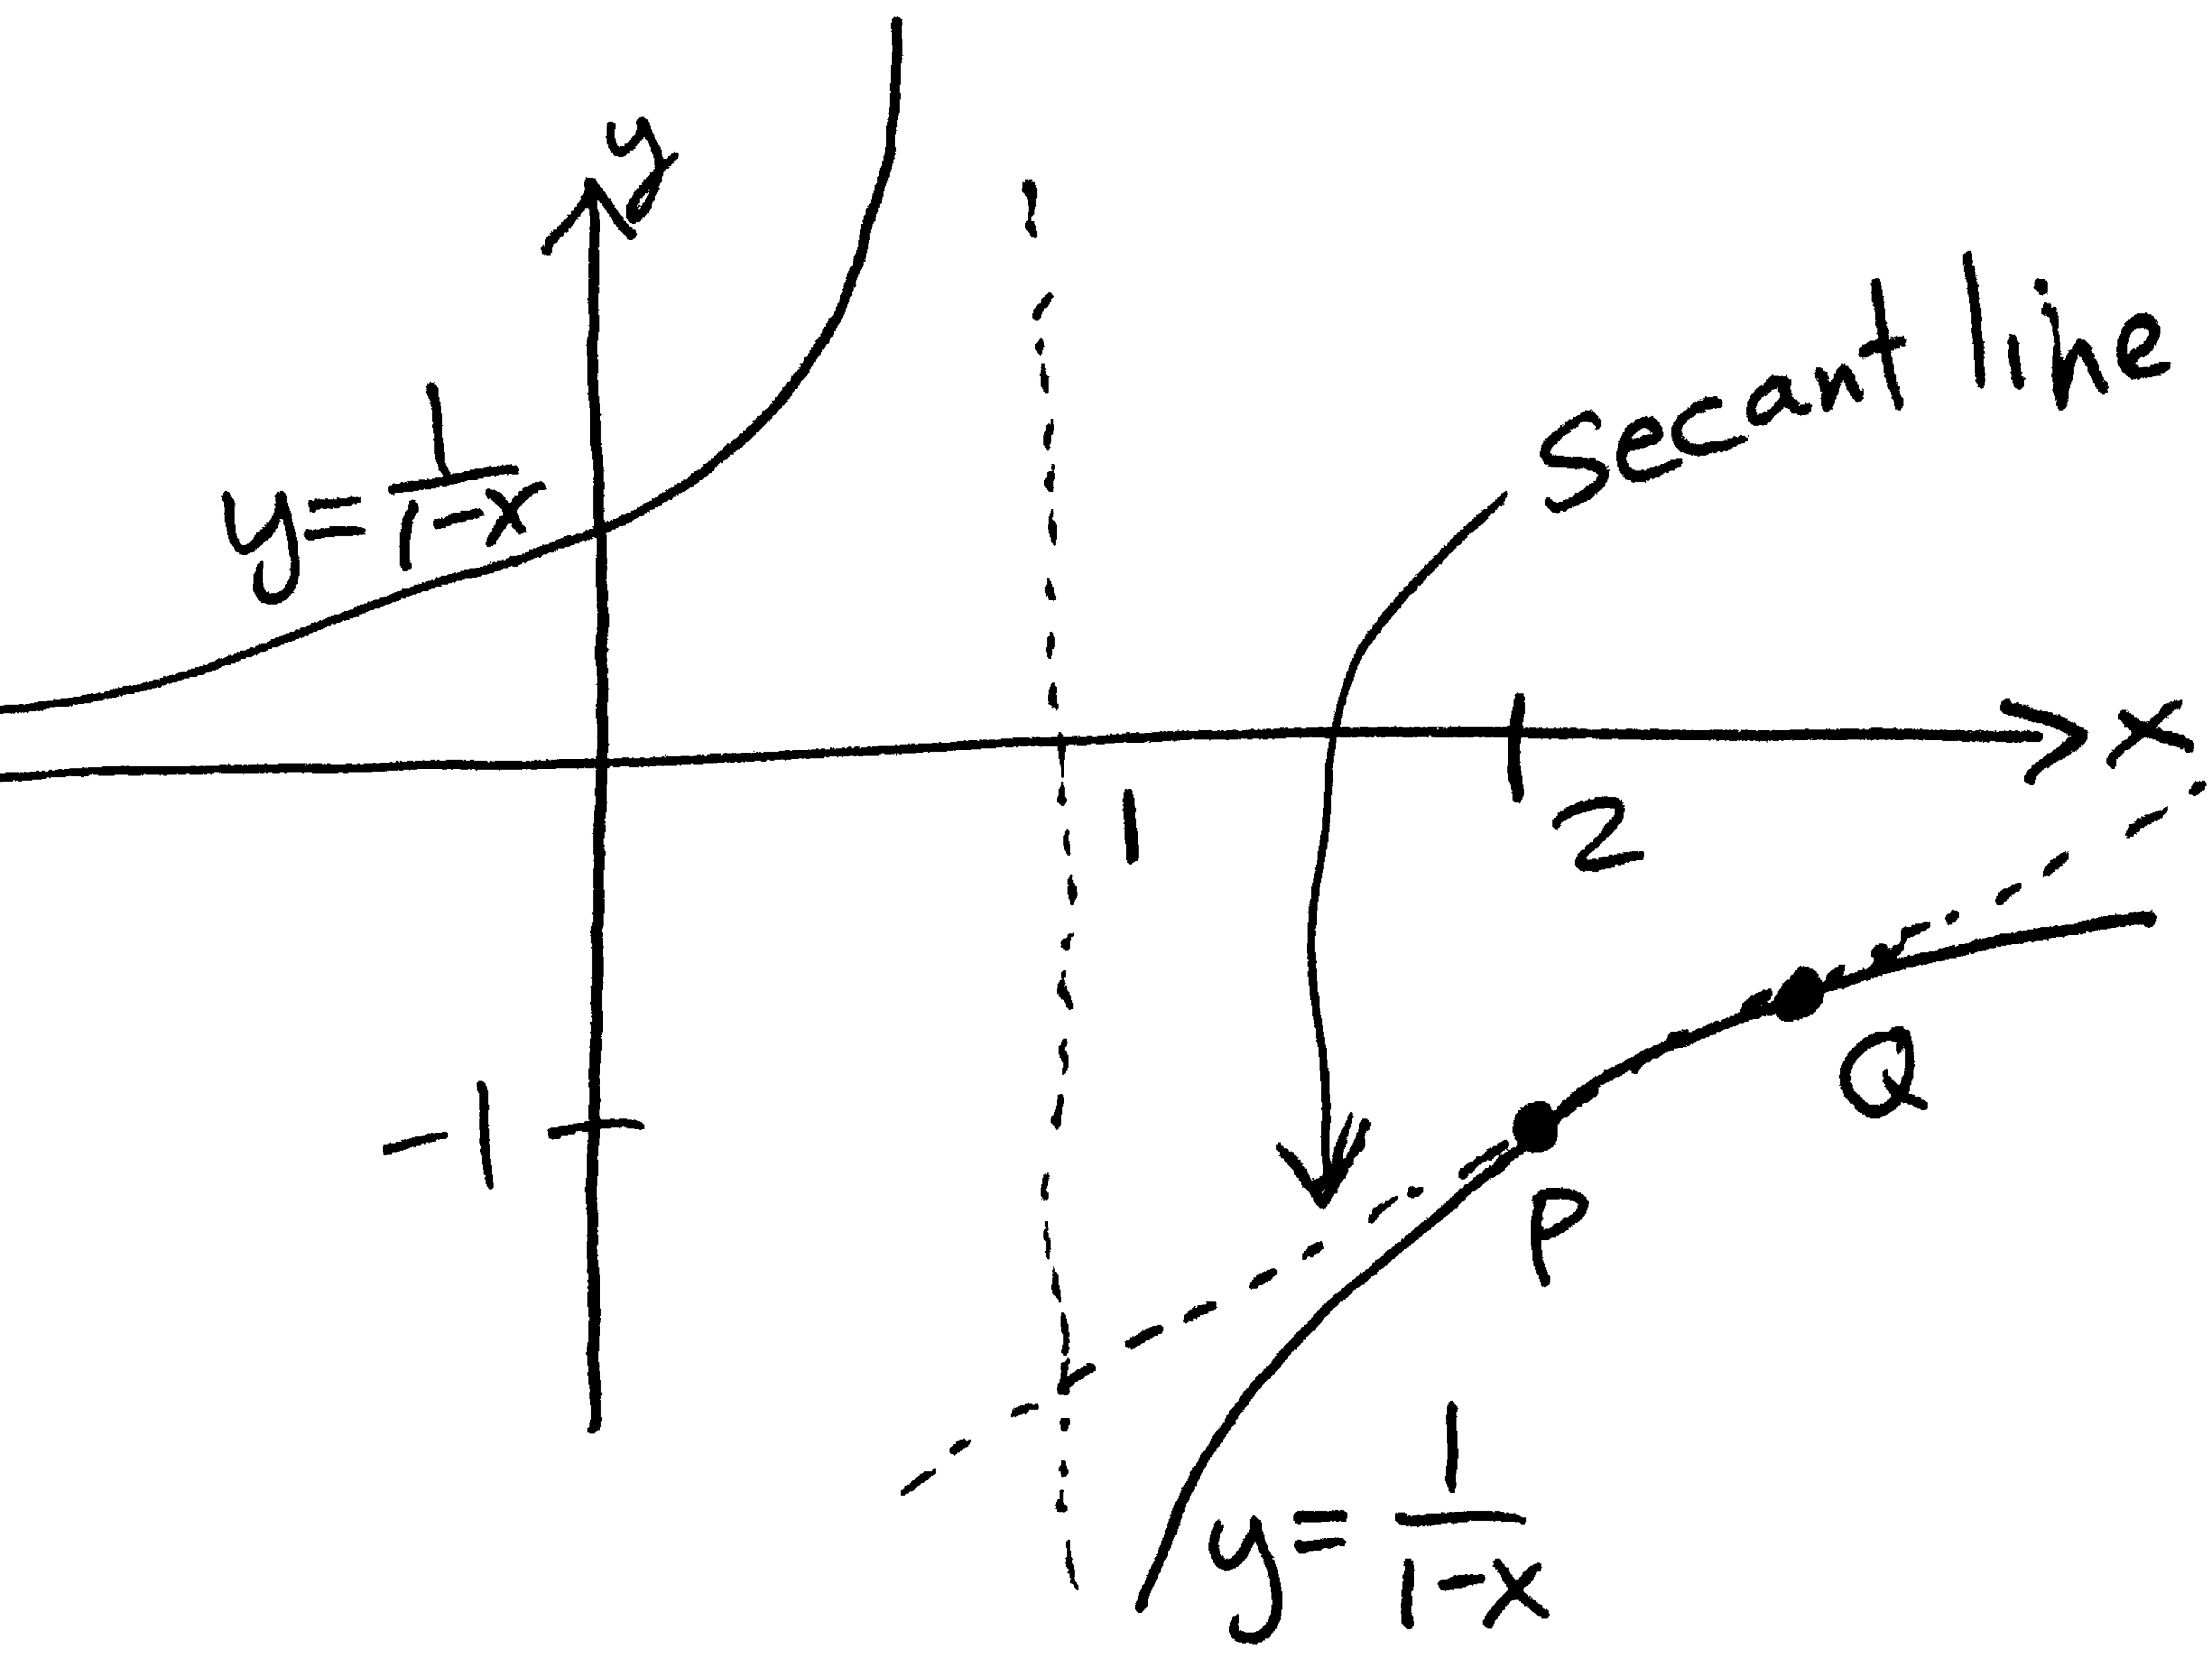
\includegraphics[align=t,width=0.45\textwidth]{secantgraph}

\bigskip
    \item \emph{In this part $P$ is the fixed point $(2,-1)$ while $Q$ is the point given by the following $x$-values.}
    
    Let $f(x) = 1/(1-x)$.  Then:
        \renewcommand{\labelenumiii}{(\roman{enumiii})}
        \begin{enumerate}
        \item $m = (f(1.5) - f(2)) / (1.5 - 2) = 2.0$
        \item $m = (f(1.9) - f(2)) / (1.9 - 2) = 1.11$
        \item $m = (f(1.99) - f(2)) / (1.99 - 2) = 1.01$
        \item $m = (f(1.999) - f(2)) / (1.999 - 2) = 1.001$
        \item $m = (f(2.5) - f(2)) / (2.5 - 2) = 0.6667$
        \item $m = (f(2.1) - f(2)) / (2.1 - 2) = 0.9091$
        \item $m = (f(2.01) - f(2)) / (2.01 - 2) = 0.9901$
        \item $m = (f(2.001) - f(2)) / (2.001 - 2) = 0.9990$
        \end{enumerate}
% >> f = @(x) 1./(1-x);
% >> q = [1.5 1.9 1.99 1.999 2.5 2.1 2.01 2.001];
% >> m = (f(q) - f(2)) ./ (q - 2)
% m =
%   2.00000  1.11111  1.01010  1.00100  0.66667  0.90909  0.99010  0.99900
    \item Based on the above I would guess that the tangent line slope at $P(2,-1)$ is $m=1$.
    \item We have a point and a slope so the equation of line is immediate:
        $$y - (-1) = 1 (x - 2) \qquad \text{ or } \qquad y = x -3$$
    \end{enumerate}

\item  If you plot the data with a computer you see it is all close to one line.  Here we first compute the four secant line slopes:

    \renewcommand{\labelenumii}{\alph{enumii})}
    \begin{enumerate}
    \item $m=68.8$ beats/min
    \item $m=71.8$ beats/min
    \item $m=72.5$ beats/min
    \item $m=71.0$ beats/min
    \end{enumerate}

We can say with some confidence that the heart monitor should report a number between $69$ and $72$.  My choice for best estimate averages the secant slopes from a) and b):
    $$m = \frac{1}{2} (68.8+71.8) = 70.3 \,\,\text{beats/min}$$
\end{enumerate}


\end{document}
